\documentclass{beamer}
\usepackage{workshop}

\begin{document}

\title{Introduction to Python 2}
\date{May 2015}
\author{Chang Y. Chung}
\institute{Office of Population Research}

% -----------------------------------------------
{\setbeamertemplate{footline}{}
\begin{frame}[noframenumbering]
%{\color{red}D R A F T}
\titlepage
\end{frame}}

% -----------------------------------------------
\begin{frame}[fragile]
\frametitle{Algorithms + Data Structures = Programs}
\begin{itemize}
\item<1-> Niklaus Wirth (1976)\cite{Wirth1976}
\item<2-> Python's built-in data structures include:
\begin{itemize}
  \item Lists
  \item Dictionaries
  \item Tuples
\end{itemize}
\item<3-> We will also briefly talk about:
\begin{itemize}
  \item Classes
  \item Exception Handling
\end{itemize}
\end{itemize}

\begin{textblock}{5}(11.5,5)
  \visible<1->{
    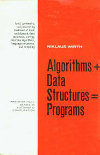
\includegraphics[width=2.5cm]{wirth.png}
  }
\end{textblock}
\end{frame}

% -----------------------------------------------
\begin{frame}[fragile]
\frametitle{List}
\begin{itemize}
\item Ordered (indexed) collection of arbitrary objects.
\item Mutable -- may be changed in place.
\end{itemize}
\end{frame}

% -----------------------------------------------
\begin{frame}[fragile]
\frametitle{List}
\begin{itemize}
\item Ordered collection of arbitrary objects.
\begin{lstlisting}[escapechar=\%]
L = []                  # a new empty list
L = list()              # ditto

L = [1, 2.5, "abc", [56.7, 78.9]]
print len(L)            # 4
print L[1]              # 2.5 (zero-based)
print L[3][0]           # 56.7

for x in L:
    print x
# 1
# 2.5
# "abc"
# [56.7, 78.9]

print "abc" in L, L.count("abc"), L.index("abc")
# True 1 2
\end{lstlisting}
\end{itemize}
\end{frame}

% -----------------------------------------------
\begin{frame}[fragile]
\frametitle{List}
\begin{itemize}
\item Mutable -- may be changed in place.
\begin{lstlisting}
L = []
L.append(5)
print L            # [5]

L[0] = 23
print L            # [23]

M = [87, 999]
L.extend(M)        # or L += M
print L            # [23, 87, 999]

del L[2]
print L            # [23, 87]
\end{lstlisting}
\end{itemize}
\end{frame}

% -----------------------------------------------
\begin{frame}[fragile]
\frametitle{List}
\begin{itemize}
\item<1-> More examples.
\begin{lstlisting}
def squares(a_list):
    s = []
    for el in a_list:
        s.append(el ** 2)
    return s

sq = squares([1,2,3,4])
print sq, sum(sq)
# [1, 4, 9, 16] 30
\end{lstlisting}
\item<2-> Aliasing vs copying
\begin{lstlisting}
L = [1,2,3,4]
M = L          # aliasing
L[0] = 87
print M        # [87, 2, 3, 4]

L = [1,2,3,4]
M = list(L)    # (shallow) copying. M = L[:] also works
L[0] = 87
print M        # [1,2,3,4]
\end{lstlisting}
\end{itemize}
\end{frame}

% -----------------------------------------------
\begin{frame}[fragile]
\frametitle{Quiz}
\begin{itemize}
\item Given a list,
\begin{lstlisting}
L = [1, 2, [3, 4], 5, "xyz"]
\end{lstlisting}
evaluate the following expressions:
\begin{lstlisting}[escapechar=\%]
L[1] == 1
len(L) == 5
L[2] == 3, 4

[3] in L
L.index("xyz") == 4
L[%\--1%] == "xyz"
L[%\--1%][%\--1%] == "z"

any([1, 2, 3]) == True
L[9] == None
len([0,1,2,]) == 3
\end{lstlisting}
\end{itemize}
\end{frame}

% -----------------------------------------------
\begin{frame}[fragile]
\frametitle{Quiz}
\begin{itemize}
\item<1-> Write a function that, given a list
    of integers, returns a \emph{new} list of odd numbers
    only. For instance, given the list, \lstinline{[0,1,2,3,4]},
    this function should return a new list,
    \lstinline{[1,3]}.

    (Hint: Create a new empty list. Loop over the
     old one appending only odd numbers into the new one.
     Return the new one.)
\item<2-> An answer.
\begin{lstlisting}
def only_odd(a_list):
    L = []
    for el in a_list:
        if el % 2 == 1:
            L.append(el)
    return L

print only_odd([0, 1, 2, 3, 4])
# [1, 3]
\end{lstlisting}
\end{itemize}
\end{frame}

% -----------------------------------------------
\begin{frame}[fragile]
\frametitle{Quiz (cont.)}
\begin{itemize}
\item (tricky) Write a function similar to the previous one.
    This time, however, do not return a new list.
    Just modify the given list so that it has only
    the odd numbers.

    (Hint: \lstinline{del L[0]} removes
    the first element of the list, \lstinline{L})
\end{itemize}
\end{frame}

% -----------------------------------------------
\begin{frame}[fragile]
\frametitle{Slice index}
\begin{itemize}
\item Applies to any sequence types, including
      \lstinline{list}, \lstinline{str},
      \lstinline{tuple}, \ldots.
\item Has three (optional) parts separated 
      by a colon (:),
      \lstinline{start : end : step}, indicating
      \lstinline{start} through but not past
      \lstinline{end}, by \lstinline{step}; Indices
      point \emph{in-between} the elements.
\begin{lstlisting}
    +---+---+---+---+---+---+
    | p | y | t | h | o | n |
    +---+---+---+---+---+---+
    0   1   2   3   4   5   6
   -6  -5  -4  -3  -2  -1
\end{lstlisting} 
\item Examples:
\begin{lstlisting}[escapechar=\%]
L = ["p", "y", "t", "h", "o", "n"]
print L[:2]        # ["p", "y"] first two
print L[1:3]       # ["y", "t"]
print L[0:5:2]     # ["p", "t", "o"]
print L[%\--1%]        # n  the last element
print L[:]         # ["p", "y", "t", "h", "o", "n"] a (shallow) copy
print L[3:]        # ["h", "o", "n"]
print L[%\--2%:]       # ["o", "n"] last two
print L[::%\--1%]      # ["n", "o", "h", "t", "y", "p"] reversed
\end{lstlisting}
\end{itemize}
\end{frame}

% -----------------------------------------------
\begin{frame}[fragile]
\frametitle{Quiz}
\begin{itemize}
\item<1-> Suppose that you collect
      friendship network data among six children,
      each of whom we identify with a number: 0, 1,
      \ldots, 5.
      The data are represented as a list of lists,
      where each element list
      represents the element child's friends.
\begin{lstlisting}
L = [[1, 2], [0, 2, 3], [0, 1], [1, 4, 5], [3, 5], [3]]
\end{lstlisting}
      For instance, the kid 0 friends with
      the kids 1 and 2, since
      \lstinline{L[0] == [1, 2]}
      Calculate the average number of friends
      the children have. (Hint: \lstinline{len()}
      returns the list size.)
\item<2-> An answer:
\begin{lstlisting}
total = 0.0            # make total a float type
for el in L:
    total += len(el)
avg = total / len(L)
print avg
# 2.1666
\end{lstlisting}
\end{itemize}
\end{frame}

% -----------------------------------------------
\begin{frame}[fragile]
\frametitle{Quiz (cont.)}
\begin{itemize}
\item (tricky)Write a function to check
      if \emph{all} the friendship choices are
      reciprocated. It should take a 
      list like previous one and return either 
      \lstinline{True} or \lstinline{False}.
      (Hint: You may want to use a utility
       function below.)
\begin{lstlisting}
def mutual(a_list, ego, alter):
    return alter in a_list[ego] and ego in a_list[alter]
\end{lstlisting}
\end{itemize}
\end{frame}
 
% -----------------------------------------------
\begin{frame}[fragile]
\frametitle{List Comprehension}
\begin{itemize}
\item A concise way to create a list. An example:
\begin{lstlisting}
[x for x in range(5) if x % 2 == 1]       # [1, 3]
\end{lstlisting}
\item An equivalent code using the for loop:
\begin{lstlisting}
L = []
for x in range(5):
    if x % 2 == 1:
        L.append(x)                       # [1, 3]
\end{lstlisting}
\item More examples.
\begin{lstlisting}[escapechar=\%]
[x %\--% 5 for x in range(6)]                 # [-5, -4, -3, -2, -1, 0]
[abs(x) for x in [%\--%2,%\--1%,0,1]]              # [2, 1, 0, 1]
[x for x in range(6) if x == x**2]        # [0, 1]
[1 for x in [87, 999, "xyz"]]             # [1, 1, 1]
[x %\--% y for x in range(2) for y in [7, 8]]  # [-7, -8, -6, -7]
\end{lstlisting}
\end{itemize}
\end{frame}
 
% -----------------------------------------------
\begin{frame}[fragile]
\frametitle{Dictionary}
\begin{itemize}
\item<1-> A collection of key-value pairs.
\item<1-> Indexed by keys.
\item<1-> Mutable.
\item<2-> Also known as associative array, map,
      symbol table, \ldots
\item<2-> Usually implemented as a hash table.
\end{itemize}
\end{frame}
 
% -----------------------------------------------
\begin{frame}[fragile]
\frametitle{Dictionary}
\begin{itemize}
\item A collection of key-value pairs, indexed by keys.
\begin{lstlisting}
D = {}                        # an empty dictionary. D=dict() also works

D["one"] = 1                  # \{"one": 1\}   
D["two"] = 2             
print D                       # \{"one": 1, "two": 2\}

print D.keys()                # ["two", "one"] arbitrary order!
print "three" in D.keys()     # False. "three" in D also works

D = {"Apple": 116, "Big Mac": 550}

for key in ["Apple", "Orange", "Big Mac"]:
    if key in D:
        value = D[key]
        print "{0} has {1} calories".format(key, value)
    else:
        print "{0} is not found in the dictionary".format(key)
# Apple has 116 calories
# Orange is not found in the dictionary
# Big Mac has 550 calories
\end{lstlisting}
\end{itemize}
\end{frame}
 
% -----------------------------------------------
\begin{frame}[fragile]
\frametitle{Dictionary}
\begin{itemize}
\item More Dictionary examples.
\begin{lstlisting}
D = {"China": 1350, "India":1221, "US":317}
for key in D.keys():
    print "Pop of {0}: {1} mil".format(key, D[key])
# Pop of India: 1221 mil
# Pop of China: 1350 mil
# Pop of US: 317 mil

D = {[1,2]: 23}
# TypeError: unhashable type: 'list'

D = {2: [2, 3], 200: [3, 4], 95: [4, 5]} # OK
print D[2]      # [2, 3]
print D[200]    # [3, 4]
\end{lstlisting}
\end{itemize}
\end{frame}

% ----------------------------------------------- 
\begin{frame}[fragile]
\frametitle{A Data Structure}
\begin{itemize}
\item<1-> SAT has three subsections: Critical Reading,
  Mathematics, and Writing. A result of taking an
  SAT exam is three scores. 
\begin{lstlisting}
# data
SAT = {"cr":780, "m":790, "w":760}
# usage
print SAT["m"]          # 790
\end{lstlisting}
\item<2-> You can take SAT exams more than once.
\begin{lstlisting}
# data
SATs = [{"cr":780, "m":790, "w":760},
        {"cr":800, "m":740, "w":790}]
# usage
print SATs[0]           # \{"cr":780, "m":790, "w":760\}
print SATs[0]["cr"]     # 780
\end{lstlisting}
\end{itemize}
\end{frame}

% ----------------------------------------------- 
\begin{frame}[fragile]
\frametitle{More Complicated Data Structure}
\begin{itemize}
\item Hypothetical SAT data for two people: Jane and Mary.
\begin{lstlisting}
SAT = {"Jane": {"lastname": "Thompson",
                "test": [{"cr": 700, "m": 690, "w":710}] },
       "Mary": {"lastname": "Smith", 
                "test": [{"cr": 780, "m": 790, "w":760},
                         {"cr": 800, "m": 740, "w":790}] }}

print SAT["Jane"]
# \{"test": [{"cr": 700, "m": 690, "w": 710}], "lastname": "Thompson"\}

print SAT["Jane"]["lastname"]      # Thompson
print SAT["Jane"]["test"]          # [\{"cr": 700, "m": 690, "w":710\}] 
print SAT["Jane"]["test"][0]       # \{"cr": 700, "m": 690, "w": 710\}
print SAT["Jane"]["test"][0]["cr"] # 700

mary1 = SAT["Mary"]["test"][1]
print mary1["cr"]                  # 800
\end{lstlisting}
\end{itemize}
\end{frame}

% -----------------------------------------------
\begin{frame}[fragile]
\frametitle{Quiz}
\begin{itemize}
\item<1-> Make a dictionary of 2012
      SAT percentile ranks for the scores
      from 660 to 700 and for all three subsections.
      The full table is available at 
      \url{http://tinyurl.com/k38xve8}.
      Given this dictionary, say \lstinline{D},
      a lookup, \lstinline{D[660]["cr"]}
      should be evaluated to \lstinline{91}.
\item<2-> An answer.
\begin{lstlisting}
D = {700: {"cr": 95, "m": 93, "w": 96},
     690: {"cr": 94, "m": 92, "w": 95},
     680: {"cr": 93, "m": 90, "w": 94}, 
     670: {"cr": 92, "m": 89, "w": 93},
     660: {"cr": 91, "m": 87, "w": 92}}

print D[660]["cr"]      # 91
\end{lstlisting}
\end{itemize}
\end{frame}

% -----------------------------------------------
\begin{frame}[fragile]
\frametitle{Quiz (cont.)}
\begin{itemize}
\item (tricky) Write a new dictionary \lstinline{DD} such that
     we look up the subsection first and then
     the score. That is,
     \lstinline{DD["cr"][660]} should be
     evaluated to \lstinline{91}.
 
     (Hint: Start with a dictionary below.):
\begin{lstlisting}
DD = {"cr": {}, "m": {}, "w": {}}
\end{lstlisting} 
\end{itemize}
\end{frame}

% -----------------------------------------------
\begin{frame}[fragile]
\frametitle{Tuples}
\begin{itemize}
\item A sequence of values separated by commas.
\item Immutable.
\item Often automatically \emph{unpacked}.
\end{itemize}
\end{frame}

% -----------------------------------------------
\begin{frame}[fragile]
\frametitle{Tuples}
\begin{itemize}
\item A sequence of values separated by commas. Immutable.
\begin{lstlisting}
T = tuple()                        # empty tuple. T = () works also
N = (1)                            # not a tuple
T = (1, 2, "abc")                  # a tuple (1, 2, "abc")
print T[0]                         # 1
T[0] = 9                           # TypeError. immutable
\end{lstlisting}
\item Often automatically unpacked.
\begin{lstlisting}
T = (2, 3)
a, b = T                           # a is 2, b is 3
a, b = b, a                        # a and b swapped.

D = {"x": 23, "y": 46}
D.items()                          # [("y", 46), ("x", 23)]
for k, v in D.items():
    print "%s ==> %d" % (k, v)     # y ==> 46
                                   # x ==> 23
\end{lstlisting}
\end{itemize}
\end{frame}

% -----------------------------------------------
\begin{frame}[fragile]
\frametitle{Class}
\begin{itemize}
\item \lstinline{class} defines a (user-defined) type,
      a grouping of some data (properties) and 
      functions that work on the data (methods).
\item An object is an \emph{instance} of a type.
\item Examples:
\begin{itemize}
  \item \lstinline{int} is a type; \lstinline{23} is an object.
  \item \lstinline{str} a type; \lstinline{"abc"} an object.
  \item "word document file" a type;
        "my\_diary.docx" is an object
\item We have been using objects.
\end{itemize}
\end{itemize}
\end{frame}

% -----------------------------------------------
\begin{frame}[fragile]
\frametitle{Examples of Built-in Types}
\begin{itemize}
\item The \lstinline{str} type has a bunch of methods.
\begin{lstlisting}
"abc".upper()                          # ABC
"abc".find("c")                        # 2
"abc".split("b")                       # ["a", "c"]
\end{lstlisting}
\item \lstinline{open()} function returns a \lstinline{file}
      object (representing an opened file). 
\begin{lstlisting}
with open("test.txt", "w") as my_file:
    my_file.write("first line\n")
    my_file.write("second line\n")
    my_file.write("third line")

    print type(my_file)                # <type "file">
    print dir(my_file)                 # properties and methods 

my_file.write("something")             # error. I/O on closed file
\end{lstlisting}
\end{itemize}
\end{frame}

% -----------------------------------------------
\begin{frame}[fragile]
\frametitle{Class}
\begin{itemize}
\item Let's create a bank account type.
\begin{lstlisting}[escapechar=\%]
class BankAccount:

    def __init__(self, initial_balance=0):
        self.balance = initial_balance

    def deposit(self, amount):
        self.balance += amount

    def withdraw(self, amount):
        self.balance %\--%= amount
\end{lstlisting}
\item Usage examples.
\begin{lstlisting}
my_account = BankAccount(100)
my_account.withdraw(5)
print my_account.balance                 # 95

your_account = BankAccount()
your_account.deposit(100)
your_account.deposit(10)
print your_account.balance               # 110
\end{lstlisting}
\end{itemize}
\end{frame}

% -----------------------------------------------
\begin{frame}[fragile]
\frametitle{Quiz}
\begin{itemize}
\item Implement a \lstinline{Person} type(or class) which has
      three properties (\lstinline{first_name},
      \lstinline{last_name}, and \lstinline{birth_year});
      and two methods: \lstinline{full_name()} and
      \lstinline{age()}. The \lstinline{age()} method
      should take the current year
      as an argument. You may use the template below. 
\begin{lstlisting}[escapechar=\%]
class Person:
    def __init__(self, first, last, year):
        pass
    def full_name(self):
        pass
    def age(self, current_year):
        pass

# check
mr_park = Person("Jae%{\color{string}--}%sang", "Park", 1977)
print mr_park.full_name()              # Jae--sang Park
print mr_park.age(2014)                # 37 
\end{lstlisting}
\end{itemize}
\end{frame}

% -----------------------------------------------
\begin{frame}[fragile]
\frametitle{Inheritance}
\begin{itemize}
\item A mechanism for code reuse in object-oriented
      programming (OOP).
\item A subtype is a specialized basetype.
\begin{lstlisting}
import webbrowser

class CoolPerson(Person):
    def __init__(self, name, birth_year, video):
        Person.__init__(self, name, None, birth_year)
        self.video = video
    def full_name(self):
        return self.first_name
    def show_off(self):
        url = "http://www.youtube.com/watch?v={0}"
        webbrowser.open(url.format(self.video))   

# check
psy = CoolPerson("PSY", 1977, "9bZkp7q19f0")
print psy.full_name()                # PSY
print psy.age(2012)                  # 35
psy.show_off()                       # show off the style
\end{lstlisting}
\end{itemize}
\end{frame}

% -----------------------------------------------
\begin{frame}[fragile]
\frametitle{Exception Handling}
\begin{itemize}
\item An exception is raised when a (run-time) error
      occurs. By default, the script stops running 
      immediately.
\begin{lstlisting}
L = [0, 1, 2, 3]
print L[5]
# IndexError: list index out of range
\end{lstlisting}
\item \lstinline{try: ... except: ...}
      let us catch the exception and handle it.
\begin{lstlisting}
L = [0, 1, 2, 3]
try:
    print L[5]           

except IndexError:
    print "no such element"

print "next"
# no such element
# next
\end{lstlisting}
\end{itemize}
\end{frame}

% -----------------------------------------------
\begin{frame}[fragile]
\frametitle{Throwing Exception}
\begin{itemize}
\item We can raise (or throw) an exception as well.
\begin{lstlisting}
def fetch(a_list, index):
    if index >= len(a_list):
        raise IndexError("Uh, oh!")
    return a_list[index]

print fetch(L, 5)
# IndexError: Uh, oh!
\end{lstlisting}
\item Script can keep going if you catch and handle the
      exception.
\begin{lstlisting}
L = [0, 1, 2, 3]
try:
    print fetch(L, 5)  # this raises an exception 
except IndexError:
    print "an exception occurred"
print "next"
# an exception occurred
# next
\end{lstlisting}
\end{itemize}
\end{frame}

% -----------------------------------------------
\begin{frame}[fragile]
\frametitle{An Example}
\begin{itemize}
\item \lstinline{urlopen()} in \lstinline{urllib2}
      module raises
      an exception when the web page is not found.
\begin{lstlisting}
import urllib2

L = ["http://google.com",
     "http://google.com/somethingfantastic",
     "http://yahoo.com"]

# we want to open each page in turn
for url in L:
    try:
        page = urllib2.urlopen(url)
        print page.getcode()
    except urllib2.HTTPError:
        print "failed to open: {0}".format(url)

# 200  (a return code of 200 means OK)
# failed to open: http://google.com/somethingfantastic
# 200 
\end{lstlisting}
\end{itemize}
\end{frame}

% -----------------------------------------------
\begin{frame}[fragile]
\frametitle{A Data Structure Usage Example}
\begin{itemize}
\item STAN (\url{http://mc-stan.org}) is  
      a C++ library / language implementing
      Markov chain Monte Carlo sampling (NUTS, HMC).
\item STAN provides
      three application programming interfaces 
      (or API's): R, Python, and shell
\item This is an example of using the Python API,
      which is provided in a Python module, PyStan\cite{STANSite}.
\item In order to run this, you need to install: 
      Cython (\url{http://cython.org}), NumPy 
      (\url{http://www.numpy.org}), and STAN itself.
\item From PyStan doc (\url{http://tinyurl.com/olap8sx}),
      fitting the eight school model in Gelman et al.
      \cite[sec 5.5]{GelmanEtAl2003}.
\end{itemize}
\end{frame}

% -----------------------------------------------
\begin{frame}[fragile]
\frametitle{Data Structure Usage Example (cont.)}
\begin{itemize}
\item Import PyStan module and put STAN code
      in a string.
\begin{lstlisting}[escapechar=\%]
import pystan
schools_code = """
data {
    int<lower=0> J; // number of schools
    real y[J]; // estimated treatment effects
    real<lower=0> sigma[J]; // s.e. of effect estimates
}
parameters {
    real mu;
    real<lower=0> tau;
    real eta[J];
}
transformed parameters {
    real theta[J];
    for (j in 1:J)
        theta[j] <%{\color{red}\--}% mu + tau * eta[j];
}
model {
    eta ~ normal(0, 1);
    y ~ normal(theta, sigma);
}
"""
\end{lstlisting}
\end{itemize}
\end{frame}

% -----------------------------------------------
\begin{frame}[fragile]
\frametitle{Data Structure Usage Example (cont.)}
\begin{itemize}
\item cont.
\begin{lstlisting}[escapechar=\%]
schools_data = {"J": 8,
                "y": [28,  8, %{\color{black}\--}%3,  7, %{\color{black}\--}%1,  1, 18, 12],
                "sigma": [15, 10, 16, 11,  9, 11, 10, 18]}

fit = pystan.stan(model_code=schools_code, 
                  data=schools_data, %{\color{black}iter}%=1000, chains=4)

la = fit.extract(permuted=True)
mu = la["mu"] 
# do something with mu here

print str(fit)    # (nicely) print fit object
fit.plot()        # requires matplotlib
\end{lstlisting}
\item Notice that:
\begin{itemize}
\item Input data are supplied in a dictionary. 
\item \lstinline{stan()} function in the module runs
      the model.
\item The function returns a \lstinline{fit} type object, which
      has several methods including \lstinline{extract()}
      and \lstinline{plot()}.
\end{itemize}
\end{itemize}
\end{frame}

% -----------------------------------------------
\begin{frame}[fragile]
\frametitle{Data Structure Usage Example (cont.)}
\begin{itemize}
\item Output, in part
\begin{lstlisting}[escapechar=\#]
INFO:pystan:COMPILING THE C++ CODE FOR MODEL anon_model NOW.
Inference #{\color{fg}for}# Stan model: anon_model.
4 chains, each with #{\color{fg}iter}#=1000; warmup=500; thin=1; 
post-warmup draws per chain=500, total post-warmup draws=2...

         mean se_mean   sd 2.5%  25%  50%  75% 97.5% n_eff...
mu        7.8     0.2  5.1 -2.0  4.4  7.9 11.3  17.2 515.0...
tau       6.4     0.3  5.4  0.4  2.6  5.1  8.6  20.5 362.0 
eta[0]    0.4     0.0  0.9 -1.5 -0.2  0.4  1.0   2.2 597.0 
eta[1]   -0.0     0.0  0.9 -1.8 -0.6 -0.0  0.5   1.7 582.0 
...
theta[6] 10.4     0.3  6.9 -1.9  5.7  9.8 14.3  25.8 594.0 
theta[7]  8.3     0.3  7.5 -6.2  3.7  8.0 12.7  25.0 604.0 
lp__     -4.9     0.1  2.6-10.5 -6.5 -4.7 -3.2  -0.3 318.0 

Samples were drawn using NUTS(diag_e) at Thu Jan  9 17:53:
For each parameter, n_eff #{\color{fg}is}# a crude measure of effective 
#{\color{fg}and}# Rhat #{\color{fg}is}# the potential scale reduction factor on split 
convergence, Rhat=1).
\end{lstlisting}
\end{itemize}
\end{frame}

% -----------------------------------------------
\begin{frame}[fragile]
\frametitle{Data Structure Usage Example (cont.)}
\begin{itemize}
\item Plots
\begin{figure}[h]
  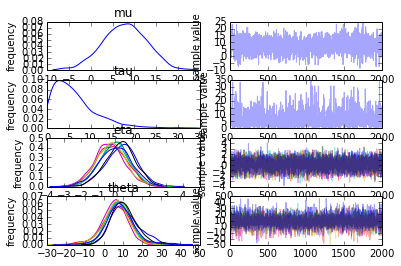
\includegraphics[width=8cm]{stan.png}
\end{figure}
\end{itemize}
\end{frame}

% -----------------------------------------------
\begin{frame}[fragile]
\frametitle{Summary}
\begin{itemize}
\item List -- An ordered collection of objects. Mutable.
\item Dictionary -- A collection of key-value pairs. Mutable.
\item Tuple -- A sequence of values separated by commas. Immutable.
\item Class -- Defines a type, a grouping of properties and methods.
\item \lstinline{try: ... except: ...} -- Catch and handle exceptions.
\end{itemize}
\end{frame}

% -----------------------------------------------
\begin{frame}%[allowframebreaks]
  \frametitle{References}
  \bibliographystyle{acm}
  \scriptsize
  \bibliography{references}
\end{frame}

\end{document}
